\documentclass[border=3pt,tikz]{standalone}
% Shared look for every TikZ figure in these notes.
% Included by each standalone figure file; also keeps the figures consistent
% with the colours used in the PDF and on the website.

\usepackage{tikz}
\usepackage{pgfplots}
\pgfplotsset{compat=1.18}
\usetikzlibrary{arrows.meta, decorations.markings, decorations.pathmorphing,
                patterns, calc, positioning}
\usepackage{amsmath}

% Series colours are the three validated categorical slots also used by the
% interactive widgets, so a path drawn in the printed notes and the same path on
% the website are the same colour. They clear the colour-vision-deficiency and
% contrast checks as a set; every path is direct-labelled as well, so colour is
% never the only thing carrying identity.
\definecolor{duPurple}{HTML}{68246D}
\definecolor{duBlue}{HTML}{2A78D6}
\definecolor{duRed}{HTML}{EB6834}
\definecolor{duGreen}{HTML}{1BAF7A}
\definecolor{duGrey}{HTML}{6B6B6B}

\tikzset{
  axisline/.style   = {-{Stealth[length=3mm]}, line width=0.7pt, black},
  path1/.style      = {duBlue,   line width=1.1pt},
  path2/.style      = {duRed,    line width=1.1pt},
  path3/.style      = {duGreen,  line width=1.1pt},
  statedot/.style   = {circle, fill=black, inner sep=1.4pt},
  arrowhead/.style  = {decoration={markings,
                        mark=at position #1 with {\arrow{Stealth[length=2.6mm]}}},
                       postaction={decorate}},
  lbl/.style        = {font=\small},
  slbl/.style       = {font=\footnotesize, duGrey},
  workfill/.style   = {duPurple, opacity=0.16},
}

\begin{document}
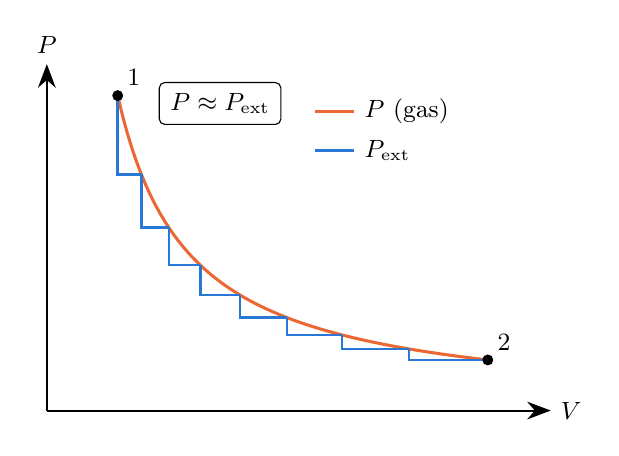
\begin{tikzpicture}
  \draw[axisline] (0,0) -- (6.4,0) node[right, lbl] {$V$};
  \draw[axisline] (0,0) -- (0,4.4) node[above, lbl] {$P$};
  % system pressure along the expansion: P = C/V
  \def\C{3.6}
  \draw[path2] plot[domain=0.9:5.6, samples=80] (\x, {\C/\x});
  % external pressure: a staircase just below it (one small mass removed per step)
  \foreach \a/\b in {0.9/1.2,1.2/1.55,1.55/1.95,1.95/2.45,2.45/3.05,3.05/3.75,3.75/4.6,4.6/5.6} {
    \draw[path1, line width=0.9pt] (\a,{\C/\a}) -- (\a,{\C/\b}) -- (\b,{\C/\b});
  }
  \node[statedot] at (0.9,{\C/0.9}) {}; \node[lbl, above right=0pt] at (0.9,{\C/0.9}) {1};
  \node[statedot] at (5.6,{\C/5.6}) {}; \node[lbl, above right=0pt] at (5.6,{\C/5.6}) {2};
  % legend
  \draw[path2] (3.4,3.8) -- (3.9,3.8) node[right, lbl, black] {$P$ (gas)};
  \draw[path1] (3.4,3.3) -- (3.9,3.3) node[right, lbl, black] {$P_\text{ext}$};
  \node[lbl, draw, rounded corners=2pt, inner sep=4pt] at (2.2,3.9) {$P \approx P_\text{ext}$};
\end{tikzpicture}
\end{document}
